\documentclass[12pt]{article}
\usepackage[margin=1in]{geometry}
\usepackage{amsmath,amssymb}
\usepackage{listings}
\usepackage{xcolor}
\usepackage{tikz}
\usetikzlibrary{trees,positioning,arrows.meta,shapes.geometric}

\lstset{
  breaklines=true,
  basicstyle=\small\ttfamily,
  columns=fullflexible,
  frame=single,
  breakatwhitespace=true,
  keywordstyle=\color{blue}\bfseries,
  commentstyle=\color{gray},
  stringstyle=\color{orange}
}

\begin{document}

\title{CPSC 223 Midterm \#2: In‑Depth Study Notes}
\author{Your Name}
\date{}
\maketitle

\tableofcontents
\newpage

\section{Hash Tables}
\subsection*{Concept \& Motivation}
A \emph{hash table} stores key–value pairs in an array of size \(m\).  A \emph{hash function} \(h(k)\) maps each key \(k\) to an index in \(\{0,\dots,m-1\}\).  With \(n\) elements, the \emph{load factor} \(\alpha = n / m\) governs performance:
\[
  \text{Average cost of lookup/insert/delete} = \Theta\bigl(1 + \alpha\bigr)\,.
\]
To keep operations \(O(1)\) amortized, maintain \(\alpha = O(1)\) by resizing when \(\alpha\) exceeds a threshold (e.g.\ 0.75).

\subsection*{Collision Resolution}
\begin{description}
  \item[Separate chaining:] Each bucket holds a linked list (or dynamic array) of entries.
    \[
      \text{Cost} = \Theta\bigl(1 + \alpha\bigr)\,.
    \]
  \item[Open addressing:] All entries live in the array; on collision probe:
    \begin{itemize}
      \item \textbf{Linear probing:} \(h_i(k) = (h(k) + i)\bmod m\).
      \item \textbf{Quadratic probing:} \(h_i(k) = (h(k) + c_1 i + c_2 i^2)\bmod m\).
      \item \textbf{Double hashing:} \(h_i(k) = (h(k) + i\cdot h'(k))\bmod m\).
    \end{itemize}
    Expected probes \(\approx 1/(1-\alpha)\).
\end{description}

\subsection*{Resizing}
When \(\alpha > \alpha_{\max}\) (e.g.\ 0.75), allocate new table of size \(\approx 2m\) and rehash all \(n\) keys in \(\Theta(n)\).  This yields amortized \(\Theta(1)\) insertion cost.

\subsection*{Example: Separate Chaining}
\begin{lstlisting}[language=C]
#define TABLE_SIZE 101

typedef struct Node {
    int key;
    int value;
    struct Node *next;
} Node;

Node* table[TABLE_SIZE];

unsigned int hash(int key) {
    return (unsigned)key % TABLE_SIZE;
}

void ht_insert(int key, int value) {
    unsigned idx = hash(key);
    Node* n = malloc(sizeof *n);
    n->key = key; n->value = value;
    n->next = table[idx];
    table[idx] = n;
}

Node* ht_search(int key) {
    unsigned idx = hash(key);
    for (Node* cur = table[idx]; cur; cur = cur->next)
        if (cur->key == key) return cur;
    return NULL;
}
\end{lstlisting}

\subsection*{Diagram: Separate Chaining Bucket}
\begin{center}
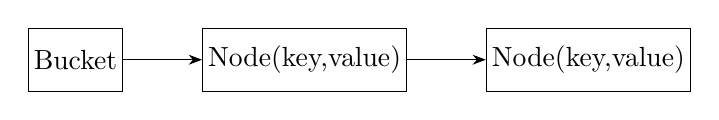
\begin{tikzpicture}[node distance=1cm, every node/.style={draw,rectangle,minimum height=8mm,inner sep=2pt}]
  \node (bucket) {Bucket};
  \node[right=of bucket] (n1) {Node(key,value)};
  \node[right=of n1] (n2) {Node(key,value)};
  \draw[-Stealth] (bucket) -- (n1);
  \draw[-Stealth] (n1) -- (n2);
\end{tikzpicture}
\end{center}

\newpage
\section{Binary Search Trees (BST)}
\subsection*{Invariant}
For every node \(x\):
\[
  \forall\,y\in\text{left}(x):\,y.\mathit{key} < x.\mathit{key},\quad
  \forall\,z\in\text{right}(x):\,z.\mathit{key} > x.\mathit{key}.
\]
If the tree has height \(h\), operations run in \(O(h)\).  In the average case \(h \approx \log n\); in the worst case \(h = n\).

\subsection*{Operations}
\begin{itemize}
  \item \textbf{Search:} Compare at current node, recurse left or right.
  \item \textbf{Insert:} BST‑search until a \texttt{NULL}, then link a new node.
  \item \textbf{Delete:} Three cases:
    \begin{enumerate}
      \item Leaf: remove directly.
      \item One child: link parent to child.
      \item Two children: replace key with in‑order successor (minimum of right subtree), then delete that node.
    \end{enumerate}
\end{itemize}

\subsection*{Example Code}
\begin{lstlisting}[language=C]
typedef struct BSTNode {
    int key;
    struct BSTNode *left, *right;
} BSTNode;

BSTNode* bst_search(BSTNode* r, int k) {
    if (!r || r->key == k) return r;
    if (k < r->key) return bst_search(r->left, k);
    else            return bst_search(r->right, k);
}

BSTNode* bst_insert(BSTNode* r, int k) {
    if (!r) {
        BSTNode* n = malloc(sizeof *n);
        n->key = k; n->left = n->right = NULL;
        return n;
    }
    if (k < r->key) r->left  = bst_insert(r->left, k);
    else if (k > r->key) r->right = bst_insert(r->right, k);
    return r;
}
\end{lstlisting}

\subsection*{Diagram: BST Example}
\begin{center}
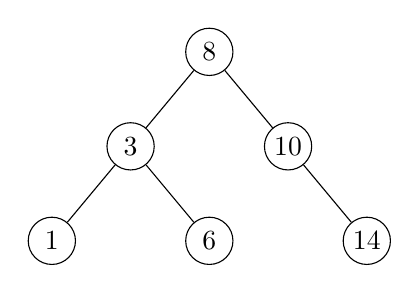
\begin{tikzpicture}[level distance=1.2cm,sibling distance=2cm,
  every node/.style={circle,draw,minimum size=6mm,inner sep=0pt}]
  \node {8}
    child { node {3}
      child { node {1} }
      child { node {6} }
    }
    child { node {10}
      child[missing]
      child { node {14} }
    };
\end{tikzpicture}
\end{center}

\newpage
\section{AVL Trees}
\subsection*{Balance Factor}
For node \(x\):
\[
  \mathit{bf}(x) = \text{height}(x.\mathrm{left}) - \text{height}(x.\mathrm{right}),\quad
  |\mathit{bf}(x)| \le 1.
\]
Insertion or deletion may violate this; if \(|\mathit{bf}(x)| = 2\), we perform rotations.

\subsection*{Rotations}
\paragraph{Right Rotation (LL Case)}
Applicable when \(\mathit{bf}(y)=+2\) and \(\mathit{bf}(y.\mathrm{left})\ge0\).
\[
  \begin{aligned}
    &x = y.\mathrm{left},\quad T_2 = x.\mathrm{right},\\
    &x.\mathrm{right} := y,\quad y.\mathrm{left} := T_2,\\
    &\text{update heights of \(y\), then \(x\)}.
  \end{aligned}
\]
\begin{lstlisting}[language=C]
AVLNode* rightRotate(AVLNode* y) {
    AVLNode* x  = y->left;
    AVLNode* T2 = x->right;
    // Perform rotation
    x->right = y;
    y->left  = T2;
    // Update heights
    y->height = 1 + max(height(y->left), height(y->right));
    x->height = 1 + max(height(x->left),      height(x->right));
    return x;  // new root
}
\end{lstlisting}

\subsection*{Diagram: Right Rotation}
\begin{center}
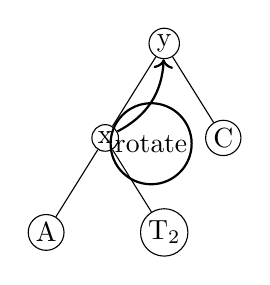
\begin{tikzpicture}[baseline=(y.base),level distance=1.2cm,
  sibling distance=1.5cm,nodes={circle,draw,inner sep=1pt}]
  \node (y) {y}
    child { node (x) {x}
      child { node {A} }
      child { node (T2) {T$_2$} }
    }
    child { node {C} };
  \draw[->,thick] (x) to[bend right] node[midway,below] {rotate} (y);
\end{tikzpicture}
\quad$\Longrightarrow$\quad
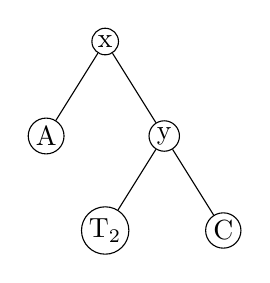
\begin{tikzpicture}[level distance=1.2cm,sibling distance=1.5cm,
  nodes={circle,draw,inner sep=1pt}]
  \node {x}
    child { node {A} }
    child { node {y}
      child { node {T$_2$} }
      child { node {C} }
    };
\end{tikzpicture}
\end{center}

\paragraph{Left Rotation (RR Case)}  
Mirror of right rotation when \(\mathit{bf}(y)=-2\) and \(\mathit{bf}(y.\mathrm{right})\le0\):
\begin{lstlisting}[language=C]
AVLNode* leftRotate(AVLNode* x) {
    AVLNode* y  = x->right;
    AVLNode* T2 = y->left;
    y->left  = x;
    x->right = T2;
    x->height = 1 + max(height(x->left),  height(x->right));
    y->height = 1 + max(height(y->left),  height(y->right));
    return y;
}
\end{lstlisting}

\paragraph{Double Rotations}
\begin{itemize}
  \item \textbf{Left–Right (LR) Case:} \(\mathit{bf}(y)=+2\) and \(\mathit{bf}(y.\mathrm{left})=-1\):
    \(\text{leftRotate}(y.\mathrm{left});\) then \(\text{rightRotate}(y);\).
  \item \textbf{Right–Left (RL) Case:} \(\mathit{bf}(y)=-2\) and \(\mathit{bf}(y.\mathrm{right})=+1\):
    \(\text{rightRotate}(y.\mathrm{right});\) then \(\text{leftRotate}(y);\).
\end{itemize}

\subsection*{Insertion Algorithm}
\begin{enumerate}
  \item Insert as in a regular BST.
  \item On unwind, update each ancestor’s height and compute \(\mathit{bf}\).
  \item At first unbalanced node, apply the appropriate single or double rotation.
\end{enumerate}
All steps cost \(O(\log n)\).

\newpage
\section{Red–Black Trees}
\subsection*{Properties}
\begin{enumerate}
  \item Every node is \textbf{red} or \textbf{black}.
  \item The root is black.
  \item Red nodes have only black children.
  \item Every path from a node to its \(\textsf{NIL}\) leaves has the same number of black nodes (the \emph{black height}).
\end{enumerate}
These ensure height \(O(\log n)\).

\subsection*{Insertion Fix‑Up}
After inserting a red node \(z\):
\begin{description}
  \item[Case 1 (Uncle red):] Recolor parent and uncle to black, grandparent to red, then repeat fix‑up on grandparent.
  \item[Case 2 (Uncle black, Triangle):] Rotate parent toward \(z\) to form a line (converts to Case 3).
  \item[Case 3 (Uncle black, Line):] Rotate grandparent opposite direction, swap colors of parent and grandparent, finish.
\end{description}

\subsection*{Diagram: RB Insertion Case 1}
\begin{center}
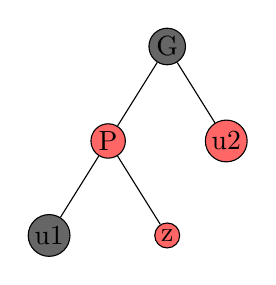
\begin{tikzpicture}[level distance=1.2cm,sibling distance=1.5cm,
  every node/.style={circle,draw,inner sep=1pt},
  rednode/.style={circle,draw,fill=red!60,inner sep=1pt},
  blacknode/.style={circle,draw,fill=black!60,inner sep=1pt}]
  \node[blacknode] (G) {G}
    child { node[rednode] (P) {P}
      child { node[blacknode] {u1} }
      child { node[rednode] (Z) {z} }
    }
    child { node[rednode] {u2} };
\end{tikzpicture}
\end{center}

\newpage
\section{$k$‑d Trees}
\subsection*{Structure \& Build}
Stores \(n\) points in \(\mathbb{R}^k\).  At depth \(d\), split on axis \(d \bmod k\).  Build in \(O(n\log n)\) via median‑of‑axis selection (e.g.\ \texttt{nth\_element}).

\begin{lstlisting}[language=C]
// Build a 2D k-d tree
kdnode* build(Point pts[], int l, int r, int depth) {
    if (l >= r) return NULL;
    int axis = depth % 2;
    int m = (l + r) / 2;
    nth_element(pts + l, pts + m, pts + r,
      [axis](const Point &a, const Point &b){
        return axis ? a.y < b.y : a.x < b.x;
      });
    kdnode* node = malloc(sizeof *node);
    node->pt = pts[m];
    node->left  = build(pts, l, m,     depth + 1);
    node->right = build(pts, m + 1, r, depth + 1);
    return node;
}
\end{lstlisting}

\subsection*{Diagram: 2D Split}
\begin{center}
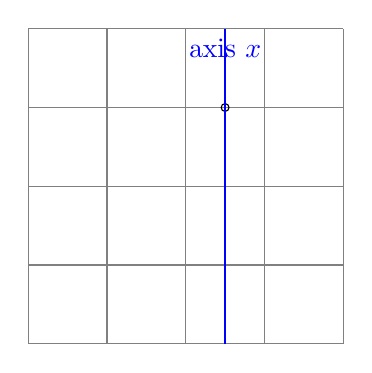
\begin{tikzpicture}[scale=1,>=Stealth,point/.style={circle,draw,inner sep=1pt}]
  \draw[thin,gray] (0,0) grid (4,4);
  \node[point] at (2.5,3) {};
  \draw[thick,blue] (2.5,0) -- (2.5,4) node[below] {axis \(x\)};
\end{tikzpicture}
\end{center}

\newpage
\section{Binary Heaps}
\subsection*{Array Representation}
A complete binary tree in an array \(A[0..n-1]\).  For index \(i\):
\[
  \text{parent}(i)=\lfloor(i-1)/2\rfloor,\quad
  \text{children}(i)=2i+1,\;2i+2.
\]
\subsection*{Operations}
\begin{itemize}
  \item \textbf{Insert:} append at end, \emph{bubble up} in \(O(\log n)\).
  \item \textbf{Extract‑Min:} swap root with last, remove last, \emph{bubble down} via \(\min\!\mathrm{Heapify}\) in \(O(\log n)\).
  \item \textbf{Build‑Heap:} call \(\min\!\mathrm{Heapify}\) from \(\lfloor n/2\rfloor\) down to 0 → \(\Theta(n)\).
\end{itemize}

\begin{lstlisting}[language=C]
// Min-heapify at index i
void minHeapify(int A[], int n, int i) {
    int l = 2*i+1, r = 2*i+2, smallest = i;
    if (l < n && A[l] < A[smallest]) smallest = l;
    if (r < n && A[r] < A[smallest]) smallest = r;
    if (smallest != i) {
        swap(&A[i], &A[smallest]);
        minHeapify(A, n, smallest);
    }
}
\end{lstlisting}

\subsection*{Diagram: Heap Tree \& Array}
\begin{center}
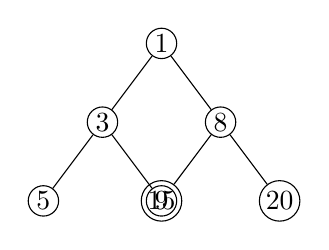
\begin{tikzpicture}[level distance=1cm,sibling distance=1.5cm,
  every node/.style={circle,draw,inner sep=1pt}]
  \node {1}
    child { node {3}
      child { node {5} }
      child { node {9} }
    }
    child { node {8}
      child { node {15} }
      child { node {20} }
    };
\end{tikzpicture}
\qquad
\begin{tabular}{|c|c|c|c|c|c|c|}
\hline
1 & 3 & 8 & 5 & 9 & 15 & 20\\\hline
\end{tabular}
\end{center}

\newpage
\section{Graphs: BFS \& DFS}
\subsection*{Representations}
\begin{itemize}
  \item \emph{Adjacency list:} \(O(V+E)\) space.
  \item \emph{Adjacency matrix:} \(O(V^2)\) space.
\end{itemize}

\subsection*{Breadth‑First Search (BFS)}
Visits vertices by increasing distance from source.  Computes shortest paths in unweighted graphs in \(O(V+E)\).
\begin{lstlisting}[language=C]
void bfs(Graph* g, int s) {
    bool seen[g->V]; int dist[g->V];
    for(int i=0;i<g->V;i++){seen[i]=false; dist[i]=INT_MAX;}
    Queue q; init(&q);
    seen[s]=true; dist[s]=0; enqueue(&q,s);
    while(!empty(&q)) {
        int u = dequeue(&q);
        for(Edge* e = g->adj[u]; e; e = e->next) {
            int v = e->to;
            if (!seen[v]) {
                seen[v] = true;
                dist[v]  = dist[u] + 1;
                enqueue(&q, v);
            }
        }
    }
}
\end{lstlisting}

\subsection*{Diagram: BFS Levels}
\begin{center}
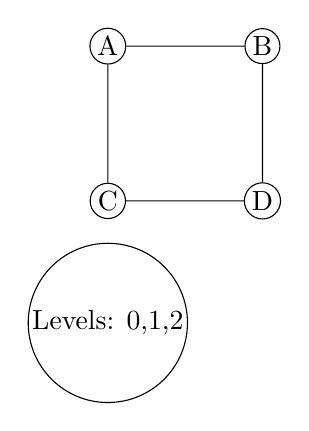
\begin{tikzpicture}[node distance=1.5cm,auto,
  every node/.style={circle,draw,inner sep=1pt}]
  \node (A) {A};
  \node[right=of A] (B) {B};
  \node[below=of A] (C) {C};
  \node[below=of B] (D) {D};
  \draw (A)--(B) (A)--(C) (B)--(D) (C)--(D);
  \node[below=0.3cm of C] {Levels: 0,1,2};
\end{tikzpicture}
\end{center}

\subsection*{Depth‑First Search (DFS)}
Explores as deep as possible before backtracking. Useful for cycle detection, topological sort, SCCs.

\subsection*{Diagram: DFS Tree}
\begin{center}
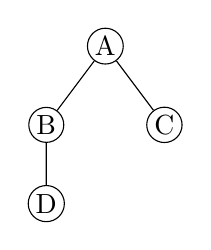
\begin{tikzpicture}[level distance=1cm,sibling distance=1.5cm,
  every node/.style={circle,draw,inner sep=1pt}]
  \node {A}
    child { node {B}
      child { node {D} }
    }
    child { node {C} };
\end{tikzpicture}
\end{center}

\newpage
\section{Shortest‑Path Algorithms}
\subsection*{BFS for Unweighted Graphs}
Since BFS explores by layers, it finds shortest paths in unweighted graphs in \(O(V+E)\).

\subsection*{Dijkstra’s Algorithm}
For non‑negative weights. Uses a min‑priority queue. Complexity \(O((V+E)\log V)\).
\begin{lstlisting}[language=C]
void dijkstra(Graph* g, int src, int dist[]) {
    bool vis[g->V];
    for(int i=0;i<g->V;i++){dist[i]=INT_MAX; vis[i]=false;}
    dist[src] = 0;
    PriorityQueue pq;
    pq.push({0,src});
    while (!pq.empty()) {
        auto [d,u] = pq.pop();
        if (d > dist[u]) continue;
        for (Edge* e = g->adj[u]; e; e = e->next) {
            int v = e->to, w = e->w;
            if (dist[u] + w < dist[v]) {
                dist[v] = dist[u] + w;
                pq.push({dist[v], v});
            }
        }
    }
}
\end{lstlisting}

\subsection*{Diagram: Dijkstra’s Relaxation}
\begin{center}
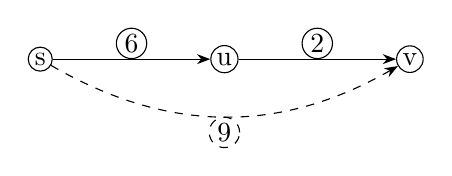
\begin{tikzpicture}[node distance=2cm,auto,
  every node/.style={circle,draw,inner sep=1pt},>=Stealth]
  \node (s) {s};
  \node[right=of s] (u) {u};
  \node[right=of u] (v) {v};
  \draw[->] (s) -- node[midway,above]{6} (u);
  \draw[->] (u) -- node[midway,above]{2} (v);
  \draw[->,dashed] (s) to[bend right] node[midway,below]{9} (v);
\end{tikzpicture}
\end{center}

\subsection*{Bellman–Ford}
Handles negative weights (no negative cycles). Relax all edges \(V-1\) times in \(O(VE)\). A \(V\)th pass detecting further relaxation signals a negative cycle.

\end{document}
